\documentclass[12pt,a4paper]{article}

% Margins.
\setlength{\oddsidemargin}{0in}
\setlength{\evensidemargin}{0in}
\setlength{\headheight}{12pt}
\setlength{\headsep}{42pt}
\setlength{\topmargin}{-54pt}
\setlength{\textwidth}{6.5in}
\setlength{\textheight}{10in}

\usepackage{amsmath}
\usepackage{float}
\usepackage{graphicx}
\usepackage[hyphens]{url}
\usepackage{hyperref}	% Clickable links to figures, references and urls.
\usepackage{datetime}
\usepackage{longtable}

% Drawing.
\usepackage{pgf}
\usepackage{tikz}

% Listings for formatting code.
\usepackage{listings}
\usepackage{textcomp}
% General options.
\lstset{breaklines=true, basicstyle=\small\ttfamily, tabsize=4, numbers=left, stepnumber=1, frame=single, showstringspaces=false, upquote=true}
% C++ specific high-lighting. Comments are 50/50 shades of green/black and strings coloured with 60/40 red/black mixture.
\lstset{language=[ISO]C++, commentstyle=\color{green!50!black}, keywordstyle=\color{blue}, stringstyle=\color{red!60!black}}

%opening
\title{\vspace{-2cm}Physics for Engineers\\Class 02\\One--Dimensional Kinematics}
\author{Attique Dawood}
\date{August 21, 2013\\[0.2cm] Last Modified: \today, \currenttime}
\begin{document}
\maketitle
Today's lecture is from sections 2.1 and 2.2 of text book \cite{Serway}.
\section{Revision}
\begin{itemize}
\item The goal of this course is to understand Maxwell's equations that govern the working of electromagnetics.
\item Scientific and engineering notations.
\end{itemize}
\section{Function}
\begin{itemize}
\item A function is a `rule' (or relationship) between two quantities.
\item Two variables, independent and dependent are associated with a function.
\item All possible values that independent variable can take is called `domain' of function.
\item All possible values that dependent variable can take is called `range' of function.
\item In the function $x(t)=2t$, $x$ is dependent variable, $t$ is independent variable and the rule is `value of $x$ is twice that of $t$' or simply $2t$.
\end{itemize}
\section{Position, Displacement and Distance}
\begin{itemize}
\item We would only cover the bare essentials of mechanics before moving on to electromagnetics.
\item In particle system we consider every object as an infinitesimally small particle no matter what the actual size is.
\item \textbf{Position} of an object (or particle) is calculated with respect to some reference, normally called `origin' in coordinate system.
\item Position--time graph of an object/particle moving back and forth.
\item \textbf{Displacement} of an object/particle is the change in its position in some time interval. As it moves from an initial position $x_i$ and ends at a final position $x_f$ the displacement is given by, $\Delta x \equiv x_f - x_i$. Note that displacement can be negative or positive. The sign shows \textit{direction} of displacement.
\item \textbf{Distance} is the total length of path followed by a particle. Distance is always positive.
\item In a football game, a player runs back and forth and may cover a distance of more than 10 km. But if we consider his displacement then it would be zero as he would eventually return to his initial position.
\item Displacement is a vector quantity and requires both a magnitude as well as direction. Since we are only working in single dimension, a $+$ or $-$ sign can represent direction for now.
\end{itemize}
\begin{figure}[H]
\centering
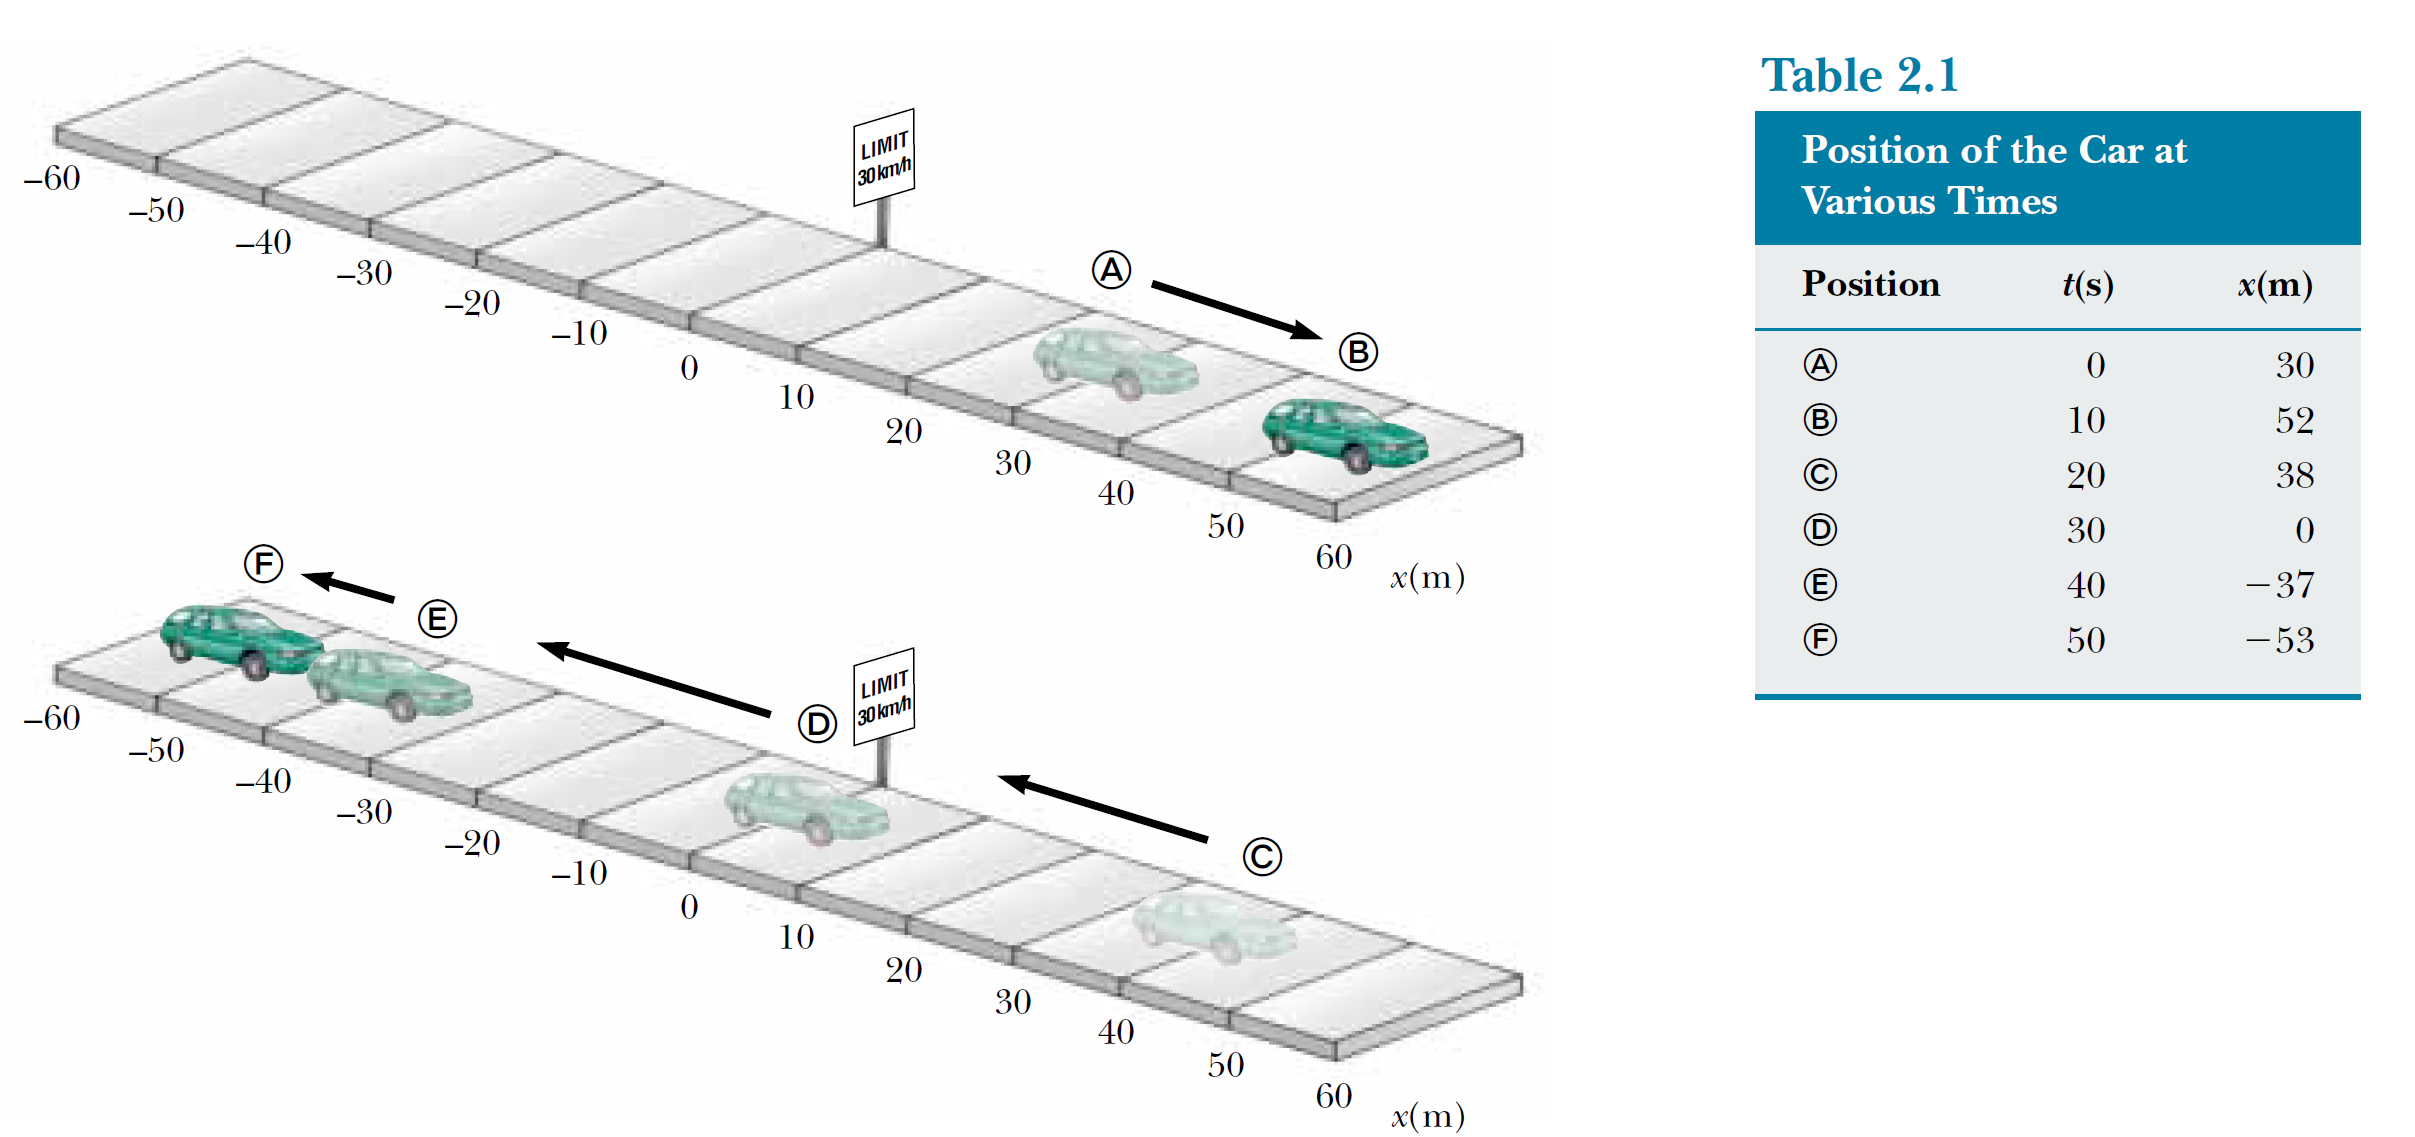
\includegraphics[scale=0.25]{Figure2-1a.png}
\caption{Car moving back and forth. Figure taken from \cite[ch. 2]{Serway}.}
\label{Car-moving-back-and-forth}
\end{figure}

\begin{figure}[H]
\centering
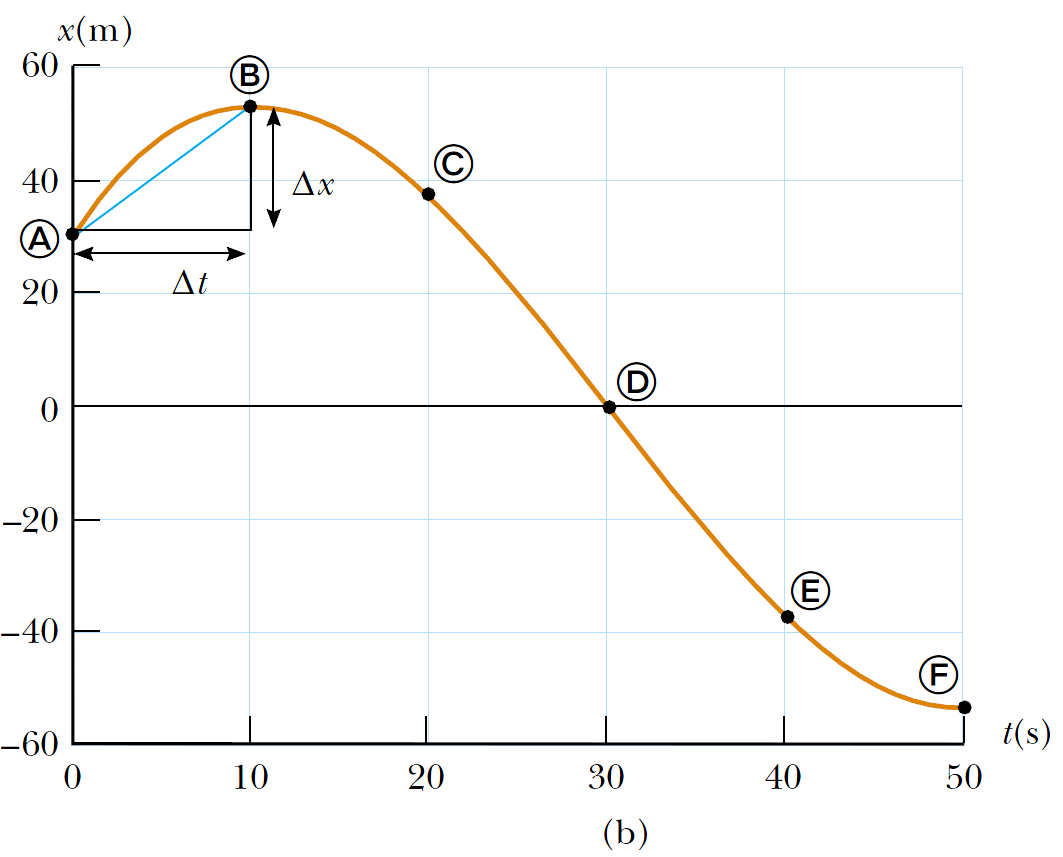
\includegraphics[scale=0.4]{Figure2-1b.png}
\caption{Position--time graph. Figure taken from \cite[ch. 2]{Serway}.}
\label{Position-time-graph}
\end{figure}
\section{Velocity and Speed}


\section{Exercises}
\noindent\textbf{Question 1:} How much distance does light travel in one year? Speed of light is $3\mathrm{e}8$ m/s.\\
\noindent\textbf{Question 2:} Express the following speeds in m/s:\\
\begin{enumerate}
\item[-] 19 km/h
\item[-] 0.030 mi/h
\item[-] 1.9 km/min
\item[-] 1000 cm/s
\item[-] 1900 km/day
\end{enumerate}
%\nocite{*}
\bibliographystyle{plain}
\bibliography{PhysicsRef}
\end{document}
